\documentclass[conference]{IEEEtran}
\IEEEoverridecommandlockouts
\usepackage{cite}
\usepackage{amsmath,amssymb}
\usepackage{graphicx}
\usepackage{booktabs}
\usepackage{multirow}
\usepackage{xcolor}
\usepackage{url}
\usepackage[hidelinks]{hyperref}

% Every number below is written by a script (scripts/01_data_stats.py, scripts/08_analyse.py).
% auto-generated by scripts; do not edit by hand
\newcommand{\NumClasses}{169}
\newcommand{\NumSurface}{316}
\newcommand{\NumThing}{130}
\newcommand{\NumStuff}{38}
\newcommand{\MeanCapLen}{10.8}
\newcommand{\ClaimsPerCaption}{2.10}
\newcommand{\ClassesPerImage}{3.85}
\newcommand{\NounCoverage}{63.5}
\newcommand{\SharePerson}{34.5}
\newcommand{\ShareThing}{44.8}
\newcommand{\ShareStuff}{20.7}

% auto-generated by scripts; do not edit by hand
\newcommand{\ThrSupport}{0.2}
\newcommand{\ThrContra}{0.05}
\newcommand{\ThrExcess}{0.0}
\newcommand{\LastK}{4}
\newcommand{\NumTests}{55}
\newcommand{\FtMinutes}{5}
\newcommand{\FtBestEpoch}{1}
\newcommand{\FtDevice}{cuda}
\newcommand{\ZsCIDEr}{0.669}
\newcommand{\FtCIDEr}{0.979}
\newcommand{\ZsSPICE}{--}
\newcommand{\FtSPICE}{--}
\newcommand{\ZsBLEU}{25.6}
\newcommand{\FtBLEU}{32.6}
\newcommand{\ZsRUOR}{14.0}
\newcommand{\FtRUOR}{15.8}
\newcommand{\ValClaims}{2{,}272}
\newcommand{\ValClaimsPerImage}{2.27}
\newcommand{\RefSupportedAll}{84.2}
\newcommand{\RefSupportedPerson}{99.1}
\newcommand{\RefSupportedThing}{75.2}
\newcommand{\RefSupportedStuff}{79.7}
\newcommand{\NoRegionPct}{1.5}
\newcommand{\VerdictSupportedPct}{9.5}
\newcommand{\VerdictContradictedPct}{30.3}
\newcommand{\VerdictUncertainPct}{60.2}
\newcommand{\AurocPerson}{0.86}
\newcommand{\AurocThing}{0.79}
\newcommand{\AurocStuff}{0.64}
\newcommand{\UnsupThingHighDet}{64.0}
\newcommand{\UnsupThingN}{258}
\newcommand{\AgreeKOne}{11.7}
\newcommand{\AgreeKFour}{11.1}
\newcommand{\AgreeKTwelve}{7.0}
\newcommand{\ExcessMedian}{0.155}
\newcommand{\ExcessPositivePct}{98.5}
\newcommand{\EntropyMedian}{0.68}
\newcommand{\AttnN}{1503}
\newcommand{\AttnImages}{1000}
\newcommand{\AttnDecoder}{fine-tuned}
\newcommand{\AttnChance}{31.8}
\newcommand{\AttnRawPoint}{26.2}
\newcommand{\AttnSinkPoint}{71.5}
\newcommand{\AttnRawTop}{0.76}
\newcommand{\AttnSinkTop}{0.61}
\newcommand{\AttnRawIoU}{12.5}
\newcommand{\AttnSinkIoU}{46.8}
\newcommand{\SinkAgreeKOne}{39.5}
\newcommand{\SinkAgreeKFour}{43.8}
\newcommand{\SinkAgreeKTwelve}{41.4}
\newcommand{\SinkVerdictSupportedPct}{37.8}
\newcommand{\SinkVerdictContradictedPct}{11.9}
\newcommand{\SinkVerdictUncertainPct}{50.3}
\newcommand{\BOneN}{689}
\newcommand{\BOneFix}{24}
\newcommand{\BOneBreak}{409}
\newcommand{\JRawProv}{0.01}
\newcommand{\PrecRawProv}{23.3}
\newcommand{\ConRawProv}{26.5}
\newcommand{\JSinkProv}{0.28}
\newcommand{\PrecSinkProv}{38.4}
\newcommand{\ConSinkProv}{9.7}
\newcommand{\JSinkCal}{0.31}
\newcommand{\PrecSinkCal}{35.3}
\newcommand{\ConSinkCal}{14.9}
\newcommand{\TsSinkCal}{0.22}
\newcommand{\TcSinkCal}{0.205}
\newcommand{\JDetProv}{0.31}
\newcommand{\PrecDetProv}{43.1}
\newcommand{\ConDetProv}{3.9}
\newcommand{\JDetCal}{0.49}
\newcommand{\PrecDetCal}{50.0}
\newcommand{\ConDetCal}{6.1}
\newcommand{\TsDetCal}{0.34}
\newcommand{\TcDetCal}{0.205}
\newcommand{\NumCheckClaims}{1{,}503}
\newcommand{\UnsupBaseRate}{23.4}
\newcommand{\BOneSinkN}{343}
\newcommand{\BOneSinkFix}{38}
\newcommand{\BOneSinkBreak}{145}
\newcommand{\BOneDetN}{128}
\newcommand{\BOneDetFix}{27}
\newcommand{\BOneDetBreak}{37}
\newcommand{\ParamsM}{23.5}
\newcommand{\InitIdentical}{all}
\newcommand{\OursRealAlt}{15.1}
\newcommand{\OursRealChanged}{65.0}
\newcommand{\OursMaskedAlt}{15.2}
\newcommand{\OursMaskedChanged}{63.3}
\newcommand{\OursFalseAlt}{0.0}
\newcommand{\OursFalseChanged}{65.0}
\newcommand{\OursCorruptPct}{12.0}
\newcommand{\OursTrainContraPct}{31.4}
\newcommand{\GateOneAttn}{0.002}
\newcommand{\GateOneFf}{0.020}
\newcommand{\SensOneMasked}{--}
\newcommand{\SensOneFalse}{--}
\newcommand{\CiderOneReal}{0.987}
\newcommand{\RuorOneReal}{15.8}
\newcommand{\AltOneReal}{15.1}
\newcommand{\KeptOneReal}{90.3}
\newcommand{\ChangedOneReal}{65.0}
\newcommand{\CiderOneMasked}{0.993}
\newcommand{\RuorOneMasked}{15.8}
\newcommand{\AltOneMasked}{15.2}
\newcommand{\KeptOneMasked}{90.9}
\newcommand{\ChangedOneMasked}{63.3}
\newcommand{\CiderOneFalse}{0.987}
\newcommand{\RuorOneFalse}{15.8}
\newcommand{\AltOneFalse}{0.0}
\newcommand{\KeptOneFalse}{90.3}
\newcommand{\ChangedOneFalse}{65.0}

% auto-generated by scripts; do not edit by hand
\newcommand{\LookAllClaims}{2{,}272}
\newcommand{\LookGtClaims}{1{,}795}
\newcommand{\LookCoverage}{79.0}
\newcommand{\LookRawPoint}{23.9}
\newcommand{\LookSinkPoint}{88.3}
\newcommand{\LookVOneRegion}{55.7}
\newcommand{\LookVTwoRegion}{75.3}
\newcommand{\LookPersonRegion}{66.4}
\newcommand{\LookDetectorRegion}{82.7}
\newcommand{\LookOracleRegion}{95.3}
\newcommand{\LookAlpha}{0.5}
\newcommand{\LookGamma}{0.5}
\newcommand{\LookGridCount}{72}
\newcommand{\LookBRegion}{74.6}
\newcommand{\LookBObjectness}{35.9}
\newcommand{\LookBUniform}{39.6}
\newcommand{\LookSwapOwn}{74.7}
\newcommand{\LookSwapOther}{22.1}
\newcommand{\LookPersonErrors}{712}
\newcommand{\LookPersonPeakErrors}{569}
\newcommand{\LookTranspose}{51.9}
\newcommand{\LookSwapPointOwn}{87.5}
\newcommand{\LookSwapPointOther}{45.4}

% auto-generated by scripts; do not edit by hand
\newcommand{\LookClosedRegion}{76.10}
\newcommand{\LookPersonSigma}{1.0}
\newcommand{\LookStuffGamma}{0.25}
\newcommand{\LookClosedPerson}{67.15}
\newcommand{\LookClosedStuff}{79.71}
\newcommand{\LookClosedThing}{83.77}
\newcommand{\LookClosedB}{75.59}
\newcommand{\LookClosedGain}{0.84}
\newcommand{\LookClosedLow}{0.16}
\newcommand{\LookClosedHigh}{1.55}
\newcommand{\LookFeatureGain}{0.70}
\newcommand{\LookFeatureLow}{0.62}
\newcommand{\LookFeatureHigh}{0.79}
\newcommand{\LookFeatureDrop}{1.69}
\newcommand{\LookRandomDrop}{0.98}
\newcommand{\LookENClaims}{1142}
\newcommand{\LookENBoxClaims}{918}
\newcommand{\LookERawError}{0.00005890}
\newcommand{\LookECaptionError}{0.170}

% auto-generated by scripts; do not edit by hand
\newcommand{\LCRLookBefore}{90.04}
\newcommand{\LCRLookAfter}{93.28}
\newcommand{\LCRSmallBefore}{4.94}
\newcommand{\LCRSmallAfter}{55.56}
\newcommand{\LCRFitImages}{2365}
\newcommand{\LCRCalImages}{635}
\newcommand{\LCRCheckJ}{0.492}
\newcommand{\LCRCheckPrecision}{0.492}
\newcommand{\LCRCheckRecall}{0.302}


\begin{document}

\title{Look--Check--Retell: Learning to Use Visual Verification Feedback for Faithful Image Captioning\\[2pt]
\large CS415 Term Project -- Progress Report}

\author{
\IEEEauthorblockN{%
\.{I}brahim G\"{o}zl\"{u}kaya (34528) \quad
Metin Caner Ayd\i{}n (34541) \quad
\.{I}brahim Billurcu (34264)\\
Zeynep Bahar Deniz (34194) \quad
Damla Kemal (34392)}
\IEEEauthorblockA{Faculty of Engineering and Natural Sciences, Saban\c{c}\i{} University, Istanbul, Turkey}
}

\maketitle

\begin{abstract}
Image captioners name objects that are not in the image, and standard caption metrics barely register it. Look--Check--Retell (LCR) lets a frozen BLIP captioner draft a caption, uses the captioner's own cross-attention to pick an image region for every object claim, has a separate frozen OWLv2 detector check that region, and feeds the resulting verification records back through a small zero-initialised gated pathway that regenerates the caption. This report covers the first half of the project. We describe the design decisions taken while implementing the method and their justification, and report the measurements obtained so far on the Flickr8k validation split: decoder fine-tuning (validation CIDEr \ZsCIDEr{} $\to$ \FtCIDEr{}), the behaviour of attention-based region selection and detector verdicts on \ValClaims{} draft claims, a sample-size analysis that changes how the primary hypothesis will be tested, and first training runs of the Retell pathway against its matched no-evidence control. Localisation is evaluated against human-drawn Flickr30k Entities boxes; claim-correctness results remain automatic reference proxies. Human correctness evaluation and the subsequent Check and Retell updates remain pending.
\end{abstract}

\begin{IEEEkeywords}
image captioning, object hallucination, visual grounding, cross-attention, verification feedback
\end{IEEEkeywords}

\section{Problem and Motivation}
\label{sec:intro}

Image captioning models write fluent sentences, and fluency hides their mistakes. A dog carrying a frisbee is described as ``a dog playing with a ball''; a park scene gains a bench that is not in the picture. Rohrbach \emph{et al.}~\cite{rohrbach2018object} showed that such \emph{object hallucinations} follow the statistics of the training captions more than the pixels, and that a model can improve on sentence-level metrics such as CIDEr while hallucinating more. For a reader who cannot see the image, for instance a screen-reader user, a wrongly named object is worse than a missing one, because nothing in the sentence signals that it should be doubted.

\textbf{Problem.} We work at the level of \emph{object claims}. A claim is a concrete noun in a caption that belongs to a fixed vocabulary $V$ (Section~\ref{sec:design-claims}). All person words (\emph{man}, \emph{girl}, \emph{people}, \dots) form a single class \emph{person} that is checked for presence only; gender and age are never verified or scored, because detector-based checks of them are unreliable and raise fairness concerns~\cite{hendricks2018women}. A claim is \emph{incorrect} if no such object is visible or if another object has been given its name. Given an image and a draft caption, we want a new caption with fewer incorrect claims that keeps the correct ones and does not lose caption quality.

\textbf{Approach.} \emph{Look--Check--Retell} (LCR) is a two-pass captioner (Fig.~\ref{fig:pipeline}). A frozen BLIP model~\cite{li2022blip} drafts a caption. \emph{Look} uses BLIP's own decoder cross-attention to pick an image region for each claim. \emph{Check} asks a separate frozen open-vocabulary detector, OWLv2~\cite{minderer2023scaling}, what that region contains and writes a small \emph{verification record}. \emph{Retell} regenerates the caption with BLIP, which now also attends to the records through a small trainable gated pathway. The detector is itself imperfect and its scores are not calibrated probabilities~\cite{guo2017calibration}, so the pathway has to learn \emph{when} evidence should change the caption; it must not copy the detector blindly.

\textbf{Research question.} Can a captioner learn to use noisy, claim-specific verification evidence to improve its captions while rejecting misleading evidence, when the checked regions are chosen by its own attention?

\textbf{Scope of this report.} The proposal fixed seven hypotheses (H1--H6 and H1b) and a 12-week plan. This report covers the first part of that plan. We describe the design decisions taken while turning the proposal into a working system and the reasons behind them (Section~\ref{sec:design}), and we report what has been measured so far (Section~\ref{sec:experiments}). All experiments use the Flickr8k training and validation splits only; the test split has not been touched, as the protocol requires. Several of our measurements use the reference captions as a stand-in for human judgment. We label every such number as a proxy, and we list what remains open in Section~\ref{sec:conclusion}.

\section{Related Work}
\label{sec:related}

\subsection{Image Captioning Models}
Neural captioning started with a CNN encoder and an LSTM decoder trained end to end~\cite{vinyals2015show}. Xu \emph{et al.}~\cite{xu2015show} added visual attention, so that each word is generated while the decoder weighs image locations, and already used the attention maps to inspect what the model ``looks at''. Bottom-up and top-down attention~\cite{anderson2018bottom} replaced the uniform grid with object regions from a detector, and Neural Baby Talk~\cite{lu2018neural} went further by generating a sentence template whose slots are filled with the classes of detected regions. Both tie words to detector output inside a single generation pass. Transformer architectures~\cite{vaswani2017attention,dosovitskiy2021image} and large-scale vision--language pre-training~\cite{radford2021learning} then became standard. BLIP~\cite{li2022blip} combines a ViT image encoder with a BERT-style~\cite{devlin2019bert} text decoder that reads image patches through cross-attention in every layer; BLIP-2~\cite{li2023blip2} and LLaVA~\cite{liu2023visual} connect frozen image encoders to large language models. We use BLIP-base because its decoder exposes explicit cross-attention over a $24\times24$ patch grid, which Look needs, and because it is small enough to train on a single GPU.

\subsection{Measuring Caption Quality and Hallucination}
Caption quality is usually reported with n-gram and scene-graph metrics computed against reference captions: BLEU~\cite{papineni2002bleu}, METEOR~\cite{banerjee2005meteor}, CIDEr~\cite{vedantam2015cider} and SPICE~\cite{anderson2016spice}, typically through the COCO caption toolkit~\cite{chen2015microsoft}; CLIPScore~\cite{hessel2021clipscore} is a reference-free alternative. None of these was designed to detect a single wrong object. CHAIR~\cite{rohrbach2018object} therefore counts generated objects that are absent from the exhaustive COCO annotations~\cite{lin2014microsoft}, per mention (CHAIR$_i$) and per sentence (CHAIR$_s$). POPE~\cite{li2023evaluating} asks a model yes/no questions about object existence and shows that frequent and co-occurring objects are hallucinated most. Dai \emph{et al.}~\cite{dai2023plausible} study how pre-training objectives and image encodings affect hallucination. ALOHa~\cite{petryk2024aloha} extends hallucination measurement to open vocabularies by matching objects extracted by a language model against reference and detected objects. All of these depend on how completely the available annotations describe the image. Flickr8k~\cite{hodosh2013framing} has five captions per image and no object annotations, so an object that no caption mentions may still be visible. This is why our primary measure is human judgment and why CHAIR on COCO is a secondary one; Section~\ref{sec:exp-check} quantifies how incomplete the references are.

\subsection{Detector-Based Correction}
A first family of methods checks a caption against an external vision model. The Cascaded Revision Network~\cite{feng2020cascaded} predicts inaccurate words and replaces them with object words from a pretrained detector, for novel-object captioning. ReFrame~\cite{adhikary2024reframe} is a rule-based plug-in that rectifies missing or incorrect objects with a Mask R-CNN detector. Woodpecker~\cite{yin2024woodpecker} extracts key concepts, validates them with a detector and a VQA model, and lets a language model rewrite the response; Visual Fact Checker~\cite{ge2024visual} lets a language model call detection and VQA tools before producing the final caption. These pipelines are training-free, which also means that the rewriting model has never been taught how reliable its tools are. HALC~\cite{chen2024halc} stays inside decoding: an open-vocabulary detector grounds each object token and the output distributions under different fields of view are contrasted. Other decoding-time methods need no detector at all: visual contrastive decoding~\cite{leng2024mitigating} contrasts predictions for the original and a distorted image, and OPERA~\cite{huang2024opera} penalises an attention pattern associated with hallucination during beam search.

\subsection{Learned Editing and Feedback}
A second family learns to revise. Show, Edit and Tell~\cite{sammani2020show} trains a model that edits an existing caption given the image. LURE~\cite{zhou2024analyzing} trains a revisor on descriptions that were corrupted synthetically according to co-occurrence, uncertainty and position; at inference it receives no external, claim-specific evidence. We borrow its synthetic-corruption idea. Volcano~\cite{lee2024volcano} trains one model to produce feedback on its own answer, revise it and decide whether to keep the revision. HELPD~\cite{yuan2024helpd} adds object- and sentence-level feedback to training and penalises decoding with an image-attention term; attention shapes the penalty but is not used to choose regions for an external check. Biten \emph{et al.}~\cite{biten2022let} feed object labels to the captioner and augment the training sentences to weaken co-occurrence bias; their labels describe the image as a whole and do not verify individual claims. This is the design that our image-level baseline B2 imitates.

\subsection{Conditioning Frozen Generators}
Parameter-efficient methods add a small number of trainable weights to a frozen model, for example adapters~\cite{houlsby2019parameter} or low-rank updates~\cite{hu2022lora}. Flamingo~\cite{alayrac2022flamingo} inserts cross-attention layers into a frozen language model and scales their output with a $\tanh$ gate initialised at zero, so that the model starts exactly at its pretrained behaviour; LLaMA-Adapter~\cite{zhang2024llama} uses a similar zero-initialised gate. We use this mechanism to inject verification records instead of images. The zero initialisation matters for our evaluation: before training, the system is identical to the baseline, so any later difference is caused by the trained pathway.

\subsection{Open-Vocabulary Detection}
Checking arbitrary caption nouns requires a detector that accepts text queries. GLIP~\cite{li2022grounded} and Grounding DINO~\cite{liu2024grounding} cast detection as phrase grounding. OWL-ViT~\cite{minderer2022simple} attaches box and class heads to a CLIP-style image encoder and scores each predicted box against text embeddings; OWLv2~\cite{minderer2023scaling} scales it up by self-training on web image--text pairs and adds an objectness score. We chose OWLv2 for an architectural reason: the image and text towers only meet in a final dot product, so the image side can be computed once and cached, and any later text query costs a matrix product (Section~\ref{sec:design-check}). Fusion-based detectors would require a new forward pass for every query set.

\subsection{Attention as a Localisation Signal}
Whether attention explains a model's output is disputed~\cite{jain2019attention}. Gradient-based alternatives exist, from Grad-CAM~\cite{selvaraju2017grad} to the relevance propagation of Chefer \emph{et al.}~\cite{chefer2021generic} for encoder--decoder transformers. For our purposes the question is narrower: does attention point at the region the word is about? Zhang \emph{et al.}~\cite{zhang2025mllms} find that large multimodal models often attend to the correct region even when their answer is wrong, and a recent preprint~\cite{sanogo2025toward} uses attention-guided crops for training-free self-correction. Whether a compact captioner such as BLIP behaves the same way is one of our hypotheses (H6). Phrase-to-region annotations that would answer it directly exist for Flickr30k~\cite{plummer2015flickr30k} but not for Flickr8k, so we have to box a sample by hand. On the other side, Geigle \emph{et al.}~\cite{geigle2024does} report that adding grounding objectives has little or no effect on hallucination in open captioning. Good grounding alone may therefore not be enough, which motivates feeding back the \emph{result} of a check in addition to its location.

\subsection{Research Gap}
Table~\ref{tab:prior} positions LCR against the closest methods. Caption editing, self-feedback and detector verification all exist. In the work we reviewed we did not find a method that \emph{trains} a captioner to regenerate its caption from external, claim-specific records whose regions are selected by its own cross-attention. We do not claim that any component is new. The contribution is the combination and its controlled evaluation: a matched control without evidence (B0+), matched controls for evidence format (B2) and for region selection (B3), and interventions that test whether correct and false evidence are used selectively.

\begin{table}[t]
\caption{Closest prior work. \emph{External}: claim-specific evidence from a separate model at inference. \emph{Own att.}: the captioner's attention selects the checked region.}
\label{tab:prior}
\centering
\footnotesize
\setlength{\tabcolsep}{3.5pt}
\begin{tabular}{@{}p{2.3cm}cccp{1.7cm}@{}}
\toprule
Method & Learned & External & Own att. & Output \\
\midrule
CRN~\cite{feng2020cascaded} & yes & yes & no & word substitution \\
ReFrame~\cite{adhikary2024reframe} & no & yes & no & rule-based fix \\
Woodpecker~\cite{yin2024woodpecker}, VFC~\cite{ge2024visual} & no & yes & no & LLM rewrite \\
HALC~\cite{chen2024halc} & no & yes & no & contrastive decoding \\
Edit\&Tell~\cite{sammani2020show}, LURE~\cite{zhou2024analyzing} & yes & no & no & learned revision \\
Volcano~\cite{lee2024volcano} & yes & no & no & self-feedback \\
HELPD~\cite{yuan2024helpd} & yes & no & no & penalised decoding \\
Biten \emph{et al.}~\cite{biten2022let} & yes & no & no & label conditioning \\
\textbf{LCR (ours)} & yes & yes & yes & regeneration \\
\bottomrule
\end{tabular}
\end{table}

\section{Design Decisions and Their Justification}
\label{sec:design}

The proposal fixed the method at the level of Fig.~\ref{fig:pipeline}. Implementing it forced a number of concrete choices. This section records each choice with its reason, and states where it refines or departs from the proposal. The current Look/Check implementation is tested separately from the historical Retell runs. New Retell training is deferred; the retained pathway below describes its architecture, not a newly evaluated correction system.

\begin{figure*}[t]
\centering
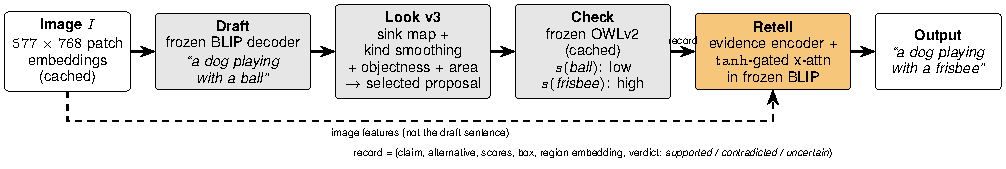
\includegraphics[width=\textwidth]{figures/pipeline.pdf}
\caption{Look--Check--Retell. Grey blocks are frozen; only the evidence encoder and the gated blocks (orange) are trained. Retell receives the image and the verification records, not the draft sentence, so it regenerates the caption; it does not edit it.}
\label{fig:pipeline}
\end{figure*}

\subsection{Frozen Captioner and Shared Visual Features}
\label{sec:design-captioner}
\textbf{Decision.} The drafting model is BLIP-base~\cite{li2022blip}, initialised from the public captioning checkpoint. On Flickr8k we fine-tune only its text decoder and keep the ViT image encoder frozen.

\textbf{Justification.} With a frozen encoder, the $577\times768$ patch embeddings of an image never change. We compute them once, store them in half precision, and every later stage reads them from disk: decoder fine-tuning, drafting, attention extraction, Retell training and all baselines. This has three consequences. (i) Every compared system sees \emph{bit-identical} visual input, which removes one source of uncontrolled variation between B0, B0+, B2, B3 and LCR. (ii) The attention grid that Look relies on keeps a fixed geometry. (iii) Training steps touch only the 12-layer decoder, so every training run in this report takes minutes on a single GPU (we used one Colab A100 for all runs). The proposal spoke of fine-tuning BLIP without saying which parts; freezing the encoder is our reading of it, and we flag it as a choice that trades a small amount of caption quality for control and speed.

\subsection{Held-Out Drafts}
\textbf{Decision.} The 6{,}000 training images are split by a seeded permutation into disjoint halves A and B of 3{,}000 images. The decoder is fine-tuned on A. Its drafts on B train the Retell pathway, and its drafts on validation and test are used for evaluation.

\textbf{Justification.} A captioner drafts images from its own training set unusually well, so the errors it makes there are neither as frequent nor of the same kind as its test-time errors. A pathway trained on such drafts would see evidence that almost always agrees with the claim. With the A/B split, Retell is trained and tested on drafts of images the captioner has not been fine-tuned on. The scripts refuse to draft a half with the decoder that was trained on it.

\subsection{Claim Vocabulary and Extraction}
\label{sec:design-claims}
\textbf{Decision.} $V$ contains \NumClasses{} classes with \NumSurface{} surface forms, curated by hand from the nouns that occur at least 30 times in the training captions. Synonyms share a class (\emph{bicycle}/\emph{bike}, \emph{couch}/\emph{sofa}); all person words form the class \emph{person}. Each class has a \emph{kind}: \emph{person}, \emph{thing} (\NumThing{} countable objects) or \emph{stuff} (\NumStuff{} amorphous regions such as \emph{water}, \emph{grass}, \emph{beach}). A caption word becomes a claim if a part-of-speech tagger marks it as a noun, it maps to a class, and it is not the modifier of a following vocabulary noun (\emph{water bottle} claims a bottle, not water). Each caption contributes at most one claim per class.

\textbf{Justification.} We first tried to build $V$ automatically from WordNet~\cite{miller1995wordnet} categories. The result was unusable: \emph{table} and \emph{forest} are filed under groups, \emph{bikini} under locations. A fixed, human-readable list is also what makes the fairness rule enforceable, since no person word can ever be ``corrected'' into another. We exclude body parts (they belong to a person or animal that is already checked), sport names that are ambiguous with the ball (\emph{football}), and placeholders such as \emph{something}. The \emph{kind} label is an addition to the proposal. A box detector cannot localise \emph{water} or \emph{snow} the way it localises a frisbee, and Section~\ref{sec:exp-check} shows that this distinction matters, so we report the kinds separately throughout.

\subsection{Look: Attention to Region}
\label{sec:design-look}
\textbf{Decision.} After drafting, the finished caption is replayed with teacher forcing. Look reads cross-attention at the position predicting the first word piece of each claim, using the four previously selected E3 heads. The caption-wide mean is subtracted before pooling and rectification, and the map is normalised. The selected heads and person smoothing/SAM rule remain frozen. This is a post-hoc, caption-contrastive map; good localisation does not by itself establish causal dependence of the prediction on that region~\cite{jain2019attention}.

\textbf{Region selection.} For a cached OWLv2 proposal $b$, attention mass and query-independent selection score are
\begin{align}
m_A(b)&=\sum_{i,j}A_{ij}\frac{|c_{ij}\cap b|}{|c_{ij}|},\\
r(b)&=\frac{m_A(b)}{\max(a(b),\epsilon)^{\alpha}}\max(o(b),\epsilon)^{\gamma},
\label{eq:lookv2}
\end{align}
where $a(b)$ is normalised area and $o(b)$ is objectness. For non-person claims, Look retains up to three finite, positive-area proposals with positive attention evidence, ranked by $r$. The old two-patch minimum side filter is removed after its B-only ablation: it excluded tight boxes of visible small objects. The area exponent remains $\alpha=\LookAlpha$; the existing kind-specific objectness exponents remain fixed. No claim-specific detector score enters this ranking. Person claims retain their SAM geometry and explicitly marked nearest-OWL-proposal score proxy.

\textbf{Justification.} Attention supplies the location, while the detector supplies object evidence there. Treating the attention map, the chosen box, and that proposal's classification feature as three separate stages exposes failures that a single end-to-end score hides. The sink correction is our caption-baseline adaptation, motivated by attention sinks~\cite{darcet2024vision}. The head selection, box ranking, and three-candidate aggregation are project choices evaluated on B, rather than claimed reproductions of a cited method.

\textbf{Independent localisation target.} Flickr30k Entities~\cite{plummer2015flickr30k} supplies human-drawn boxes for the Flickr8k images. Reference noun phrases are mapped to our vocabulary and all matching boxes are collected per class. A selected proposal succeeds when its maximum IoU with any matching box reaches the fixed threshold. This measures class-level localisation, rather than exact referent identity; claims without matching annotated boxes are counted but excluded from localisation accuracy. Pointing uses the peak patch centre; energy uses the exact geometric union of the human boxes, counting overlaps once. The boxes are used for evaluation and a small hyperparameter search on B, not model training. Test annotations are not read.

\textbf{Coordinates.} BLIP resizes the image to $384\times384$ without preserving the aspect ratio, so its patch grid is uniform in normalised image coordinates. OWLv2 pads the image to a square at the bottom or right before resizing, so its boxes are relative to a square of side $\max(W,H)$. We convert both to coordinates normalised by the original width and height. Unit tests check the conversion on landscape and portrait images, where a box covering the unpadded area must map exactly to the full image.

\subsection{Check: Cached Open-Vocabulary Verification}
\label{sec:design-check}
\textbf{Decision.} OWLv2 runs once per image. After non-maximum suppression (IoU $0.5$) we keep the 100 proposals with the highest objectness and cache, for each, the box, the objectness, the normalised 512-d class embedding $\mathbf{z}$, and two scalars: the logit shift $\beta$ and scale $\gamma$ that the class head predicts for that proposal. The probability that proposal $p$ shows class $c$ with text embedding $\mathbf{q}_c$ is then
\begin{equation}
s_p(c)=\sigma\!\big(\gamma_p\,(\mathbf{z}_p^{\top}\mathbf{q}_c+\beta_p)\big).
\label{eq:owl}
\end{equation}

\textbf{Justification.} The proposal planned to cache the class embedding only. Reading the detector's class head showed that this is not sufficient: without $\beta_p$ and $\gamma_p$ the scores cannot be reproduced. With them, Eq.~\eqref{eq:owl} gives the detector's exact output for \emph{any} later text query from the cache alone. This is what makes synthetic corruption cheap, since a corrupted label only needs a new dot product. The cache takes about 100\,kB per image.

\textbf{Verification evidence (S4).} The detector is unchanged and frozen; S4 works on its raw logits $\ell_p(c)=\gamma_p(\mathbf{z}_p^{\top}\mathbf{q}_c+\beta_p)$, the argument of Eq.~\eqref{eq:owl}. A wrong object word usually names something that looks like the true object, so the claim is scored against its rivals on the same proposal. Each class $c$ belongs to at most one hand-made set $S(c)$ of mutually exclusive names (for example dog, cat and horse; shirt, jacket and sweater). The rival-aware evidence is
\begin{equation*}
v_p(c)=\ell_p(c)-w\max\!\Big(0,\ \max_{j\in S(c)}\ell_p(j)-\ell_p(c)\Big),\qquad w=\CSRivalWeight,
\end{equation*}
and $v_p(c)=\ell_p(c)$ for a class without rivals. Let $R$ be Look's top-three proposals. The region evidence is $R_c=\max_{p\in R}v_p(c)$ and the image evidence is $X_c=\max_p v_p(c)$ over all proposals. With a per-class threshold $\tau_c$, every non-person claim receives one of five actions:
\begin{equation*}
\text{action}=\begin{cases}
\textit{skip} & \text{no candidate region, no }\tau_c\text{, or a non-visual idiom or compound (``at the camera'', ``hot dog'')},\\
\textit{keep} & R_c\ge\tau_c,\\
\textit{keep\_elsewhere} & R_c<\tau_c\le X_c,\\
\textit{replace} & X_c<\tau_c\text{ and a rival }j\in S(c)\text{ on Look's top-1 box has }\ell(j)\ge\tau_j,\ \ell(j)>\ell(c),\\
\textit{remove} & \text{otherwise.}
\end{cases}
\end{equation*}
\emph{Keep} is a supported verdict, \emph{keep\_elsewhere} and \emph{skip} are uncertain, and \emph{replace} and \emph{remove} are contradicted. Among qualifying rivals, the substitute is the one whose logit lies furthest above its class centre, the median image-level logit of its clean positives shrunk toward its kind. One attended proposal can therefore support a claim, while a contradiction requires that the claim is absent everywhere in the image; detecting the object elsewhere is reported separately rather than counted as support for the attended region. The evidence box stored with a decision is the box whose score made it: the proposal with the largest $v_p(c)$ for a keep, Look's top-1 proposal for a replacement.

\textbf{Calibration and limitations.} Thresholds use only B. Proxy positives for class $c$ are images whose references mention it at least twice, proxy negatives are images whose references never mention it, and $F_p$, $F_u$ are the distributions of $X_c$ in the two groups. Each class gets the cost-sensitive threshold
\begin{equation*}
\tau_c=\arg\max_{\tau}\big[F_u(\tau)-\lambda F_p(\tau)\big]
\end{equation*}
with one $\lambda$ for all classes; classes with fewer than two positives get no threshold and are never contradicted (\CSNoTau{} class). $\lambda=\CSLambda$ is the operating point with the highest out-of-fold false-contradiction rate on reference-supported thing claims that stays at or below \CSTarget\% in five image folds, and the final thresholds are refitted on all of B. These labels are automatic proxies: a reference need not mention every visible object, and a mention does not prove visibility. The components were found by an exploratory review on the same B folds, so the results in Section~\ref{sec:experiments} are a pre-registered reproduction, not an independent estimate. Calibration still counts reference mentions in the non-visual idioms that the live check skips; correcting this moves a few thresholds and is pending. No language prior, captioner-consistency signal, VQA or second verifier enters Check.

\subsection{Retell: Gated Evidence Pathway}
\label{sec:design-retell}
\textbf{Retained architecture; new training deferred.} An evidence encoder maps each inspected region to one 768-d token,
\begin{equation*}
\mathbf{t}=\mathrm{LN}\big(W_c\,\mathbf{w}_c+W_a\,\mathbf{w}_a+f([\mathbf{z}_r;\mathbf{g}])+\mathbf{v}_{\text{verdict}}\big),
\end{equation*}
where $\mathbf{w}_c,\mathbf{w}_a$ are BLIP's own frozen word embeddings of the claimed and alternative labels, $f$ is a two-layer MLP over the region embedding and nine scalars $\mathbf{g}$ (scores, excess mass, box geometry, a has-region flag), and $\mathbf{v}$ is a learned verdict embedding. A learned \emph{null token} is always prepended. Before each of the upper six decoder layers we insert a gated block in the style of Flamingo~\cite{alayrac2022flamingo}:
\begin{align}
\mathbf{h}&\leftarrow\mathbf{h}+\tanh(\alpha_1)\,\mathrm{XAttn}\big(\mathrm{LN}(\mathbf{h}),T\big),\\
\mathbf{h}&\leftarrow\mathbf{h}+\tanh(\alpha_2)\,\mathrm{FF}\big(\mathrm{LN}(\mathbf{h})\big),
\end{align}
with $T$ the evidence tokens and $\alpha_1=\alpha_2=0$ at initialisation. The frozen BLIP layer then runs unchanged. The pathway has \ParamsM{}\,M trainable parameters; BLIP and OWLv2 are frozen.

\textbf{Justification.} \emph{Zero-initialised gates.} Since $\tanh(0)=0$, the system starts as the frozen captioner exactly, which we verify in Section~\ref{sec:exp-gate}. Training can only move away from B0 if doing so lowers the captioning loss, and the learned gate values show directly how much each layer uses the pathway. \emph{Labels in BLIP's own embedding space.} The decoder already knows how to turn its word embeddings into output words, so expressing ``the alternative is \emph{frisbee}'' in that space makes the useful behaviour easy to learn from little data. \emph{Null token.} With it, cross-attention is defined when an image has no records, and the no-evidence control B0+ can use the identical architecture. \emph{Upper layers only.} Object identity is decided late in the decoder; restricting the pathway to six layers halves its size, which matters with only 3{,}000 training images. \emph{Regeneration.} Retell is not given the draft sentence. Draft information enters only through the records, so swapping a record and observing the output is a clean test of whether evidence is used.

\textbf{Training.} The target is one of the five reference captions with the standard captioning loss. Each record is dropped with probability $0.15$ so that the model also learns to caption without it.

\subsection{Synthetic Claim Corruption}
\textbf{Decision.} With probability $\rho$, a non-person training claim has its label replaced by a wrong one, the scores and verdict are recomputed for the same region with Eq.~\eqref{eq:owl}, and the original label joins the alternatives. As the wrong label we first take the captioner's own next-best vocabulary word at that position, provided no reference mentions it; if there is none, we fall back to a class with a similar co-occurrence context in the training captions.

\textbf{Justification.} Natural draft errors are rare, so most training records simply confirm the draft. Corruption creates records in which claim and visual evidence disagree, following LURE~\cite{zhou2024analyzing}. The proposal specified a frequently co-occurring noun. We prefer the captioner's runner-up word because hallucinations follow the language prior~\cite{rohrbach2018object}, and the runner-up is by construction the error this particular captioner was closest to making. No label tells the model to trust the evidence; the only supervision is still the reference captions.

\subsection{Matched Controls}
All trained systems share the frozen captioner, the pathway architecture, the optimiser and the number of updates, and differ only in the tokens they receive: LCR receives records for attention-selected regions; \textbf{B3} receives records for the region with the highest detector score for the claim; \textbf{B2} receives up to six image-level detector tags; \textbf{B0+} receives only the null token. B0+ is the control that matters most. Retell training shows the pathway 3{,}000 images that the captioner has not been fine-tuned on, so a caption can improve merely because of that extra data. Any claim about evidence must therefore be made relative to B0+, not to the draft B0.

\subsection{Evaluation Design}
\label{sec:design-eval}
\textbf{Paired analysis of the primary hypothesis.} H1 asks for a 15\% relative reduction of the human-verified incorrect claim rate (HICR). We computed how many claims this needs. Treating the two systems as independent samples, a two-proportion test at $\alpha=0.05$ and 80\% power needs the numbers in Table~\ref{tab:power} (left); at a draft error rate of 8\% that is \HPowerIndepEight{} claims per system, far beyond 400 annotated images. But the two systems caption the \emph{same} images and most claims are identical in both outputs. Only the claims that change carry information, which is the setting of an exact paired sign test~\cite{koehn2004statistical}. Table~\ref{tab:power} (right) simulates its power at exactly H1's effect: with 1\% of correct claims broken, a 15\% reduction at a draft error rate of 8\% requires fixing \HPowerFixEight{} of the draft errors, and then 1{,}000 traced draft claims give \HPowerEightOneK\% power and 2{,}000 give \HPowerEightTwoK\%; at 5\%, 2{,}000 claims give \HPowerFiveTwoK\% and 4{,}000 give \HPowerFiveFourK\%. These figures are optimistic in two ways. Claims of the same image are treated as independent, although they share an image and a caption, so the effective sample is smaller. And the sign test traces draft claims only, whereas HICR also counts objects that Retell adds; a system can repair draft claims and still raise HICR, so both are reported. The pilot error rate therefore decides whether H1 is testable at all. \emph{Decision:} H1 will be tested on paired, claim-traced outcomes with image-level bootstrap intervals. The final $N$ will be fixed from the pilot error rate before any system is run on test.

\textbf{Annotation tool.} We built an offline annotation page that shows each unique (image, caption) pair once, hides the system identity, shuffles items so that versions of one image are not adjacent, and asks for a label for every object noun, including nouns outside $V$. A scoring script computes HICR, fix, break and net repair rates, Cohen's $\kappa$~\cite{cohen1960coefficient} and bootstrap intervals from the exported files.

\textbf{Reproducibility.} Every number in Sections~\ref{sec:design} and~\ref{sec:experiments} is written into this document by the script that computed it; none is typed by hand.

\begin{table}[t]
\caption{Sample size for H1 (15\% relative HICR reduction, $\alpha=0.05$). Left: claims per system for an
independent two-proportion test at 80\% power. Right: simulated power of the paired sign test with $N$ traced
draft claims at exactly that effect: 1\% of correct claims are broken and the fix rate is set so that HICR falls
by 15\%. Optimistic: claims of one image are treated as independent, and objects added by Retell are not traced.}
\label{tab:power}
\centering\footnotesize
\begin{tabular}{@{}crc|cccc@{}}
\toprule
Draft error & Independent & Fix & \multicolumn{4}{c}{Paired power at $N$ claims} \\
rate $p_0$ & claims needed & rate & 500 & 1{,}000 & 2{,}000 & 4{,}000 \\
\midrule
5\% & 12{,}309 & 0.34 & 12\% & 23\% & 50\% & 82\% \\
8\% & 7{,}469 & 0.27 & 24\% & 52\% & 85\% & 99\% \\
12\% & 4{,}780 & 0.22 & 49\% & 83\% & 99\% & 100\% \\
\bottomrule
\end{tabular}
\end{table}


\section{Experiments and Preliminary Results}
\label{sec:experiments}

\subsection{Setup}
All experiments use the Flickr8k training split (halves A and B, 3{,}000 images each) and the 1{,}000-image validation split; the test split has not been read. Visual features are cached once (Section~\ref{sec:design-captioner}). Every GPU stage ran on a single Colab A100: caching BLIP and OWLv2 features for 7{,}000 images took under ten minutes, decoder fine-tuning \FtMinutes{} minutes, and one Retell training run about seven minutes. All scripts and the order in which they were run are in the project repository; the numbers in this section are inserted by the scripts that computed them.

Because human labels do not exist yet, several measurements below compare claims with the five reference captions. A claim whose class no reference mentions is called \emph{reference-unsupported}. This is a proxy, not a correctness judgement, and Section~\ref{sec:exp-check} shows how far it is from one.

\subsection{Current Look/Check Development on B}
The latest update preserves the captioner's attention maps and the frozen OWLv2 checker. On $B_{\mathrm{fit}}$ human boxes, removing the minimum-side filter raises top-three region coverage from \LCRLookBefore\% to \LCRLookAfter\%; for small annotated objects, counting a hit only when it lands on the small box itself, coverage is \LCRSmallBefore\% with the filter and \LCRSmallAfter\% without it. These are B development results, not new validation or test estimates. The selected Check uses the maximum class score across the attended candidates, with image-fold B-fit proxy precision \LCRCheckPrecision{}, wrong-claim recall \LCRCheckRecall{} and informedness \LCRCheckJ{}. Its Look selection had already seen B-fit boxes, so this is conditional Check cross-validation rather than a fully nested estimate of the whole pipeline.

There are \LCRFitImages{} B-fit and \LCRCalImages{} B-cal images. Final score scales and thresholds use only B-cal. Alternative-reference agreement remains limited and does not establish replacement correctness. The new implementation passes evidence-contract and fixed-draft live-replay checks, but the same-detector crop re-encoding experiment and new Retell training have not run. Validation was not reopened for these choices; subsequent results below retain their historical method identities.

\subsection{Drafting Captioner}
\label{sec:exp-captioner}
Table~\ref{tab:caption} compares the public BLIP-base captioning checkpoint with the same model after fine-tuning its decoder on half A for three epochs (AdamW~\cite{loshchilov2019decoupled}, learning rate $2\cdot10^{-5}$, one-cycle schedule, batch 32). Validation CIDEr peaked after the first epoch and slowly declined afterwards while the training loss kept falling (Fig.~\ref{fig:ft}), so the epoch-\FtBestEpoch{} checkpoint is the frozen captioner B0 for everything that follows. Fine-tuning mostly adapts the style of the captions to Flickr8k: drafts contain more claims (\ValClaimsPerImage{} per image instead of 1.84), while the reference-unsupported rate stays roughly where it was (\ZsRUOR\% $\to$ \FtRUOR\%). A better-scoring captioner is therefore not automatically a more faithful one, which is the observation that motivates the project~\cite{rohrbach2018object}.

\begin{table}[t]
\caption{Captioning quality on the Flickr8k validation split (1{,}000 images). Full COCO outputs are unavailable locally; BLEU-4 and CIDEr use the stored alphabetic-tokenisation scores. A dash marks an unavailable metric. 
BLEU-4, METEOR, ROUGE-L, SPICE $\times100$. RUOR: share of generated vocabulary claims that
no reference mentions (reference agreement, \emph{not} a hallucination rate).}
\label{tab:caption}
\centering\footnotesize\setlength{\tabcolsep}{3pt}
\begin{tabular}{@{}lcccccc@{}}
\toprule
Captioner & B-4 & M & R-L & CIDEr & SPICE & RUOR \\
\midrule
BLIP zero-shot & 25.6 & -- & -- & 0.669 & -- & 14.0 \\
BLIP fine-tuned on A (B0) & 32.6 & -- & -- & 0.979 & -- & 15.8 \\
\bottomrule
\end{tabular}
\end{table}


\begin{figure}[t]
\centering
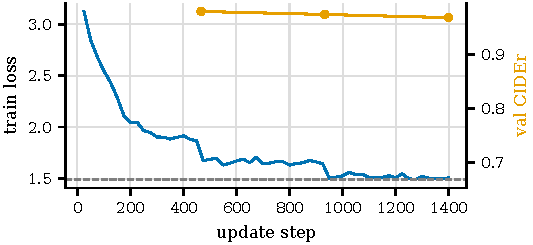
\includegraphics[width=\columnwidth]{figures/finetune_curve.pdf}
\caption{Decoder fine-tuning on half A: training loss (blue) and validation CIDEr after each epoch (orange); dashed: zero-shot CIDEr.}
\label{fig:ft}
\end{figure}

\subsection{Claims and the Limits of the Reference Proxy}
\label{sec:exp-check}
B0 produces \ValClaims{} vocabulary claims on the validation images. Of these, \RefSupportedAll\% are mentioned by at least one reference: \RefSupportedPerson\% of \emph{person} claims, \RefSupportedThing\% of \emph{thing} claims and \RefSupportedStuff\% of \emph{stuff} claims. The remaining claims are not necessarily wrong. For \UnsupThingHighDet\% of the \UnsupThingN{} reference-unsupported \emph{thing} claims, OWLv2 finds the claimed class somewhere in the image with a score above the support threshold. Many of these are plausibly real objects that the five annotators simply did not mention; the pilot labels will show how many. Conversely, the detector's best score for the claimed class separates reference-supported from reference-unsupported claims only moderately: the AUROC is \AurocPerson{} for persons, \AurocThing{} for things and \AurocStuff{} for stuff. Two conclusions follow. First, reference agreement cannot stand in for correctness, which confirms the decision to use human judgement as the primary measure. Second, the detector is markedly weaker on amorphous \emph{stuff} classes, which justifies reporting the three kinds separately.

\subsection{Look: Is Cross-Attention a Usable Localisation Signal?}
\label{sec:exp-look}
We now evaluate against human-drawn Flickr30k Entities boxes, independently of the detector's class predictions. Of \LookAllClaims{} validation claims, \LookGtClaims{} have matching boxes (\LookCoverage\%). Table~\ref{tab:look-human} separates changes to the map from changes to the region rule. The B3 class-conditioned detector and the proposal oracle are references, not alternative sources for the captioner's map.

\textbf{Map and region gains.} With v1 region selection held fixed, subtracting caption-wide attention raises pointing from \LookRawPoint\% to \LookSinkPoint\% and region accuracy to \LookVOneRegion\%. Keeping that sink map fixed, v2 raises region accuracy to \LookVTwoRegion\%; the detector reference reaches \LookDetectorRegion\%, while the candidate-pool oracle reaches \LookOracleRegion\%. The original region-rule grid contained \LookGridCount{} configurations, chosen on B before validation reporting. Corrected energy metrics integrate the actual union of boxes rather than taking the maximum per-box patch coverage. No model or region configuration was changed to obtain this measurement correction.

\begin{table}[t]
\caption{Human-box localisation on validation (\LookGtClaims{} claims). All entries are percentages.
Energy uses the exact union of annotated boxes. Pointing and energy share the map; region accuracy
also depends on the proposal rule.}
\label{tab:look-human}
\centering\footnotesize
\begin{tabular}{@{}lrrr@{}}
\toprule
Map + region rule & Pointing & Energy & Region \\
\midrule
Raw + v1 & 23.9 & 35.8 & 12.9 \\
Sink + v1 & 88.3 & 73.2 & 55.7 \\
Sink + v2 & 88.3 & 73.2 & 75.3 \\
\bottomrule
\end{tabular}
\end{table}

\begin{table}[t]
\caption{Look v2 region accuracy by kind, against any matching human box at IoU $\geq 0.5$.
B3 uses the claimed class score; oracle asks whether any eligible proposal succeeds. Percentages.}
\label{tab:look-kind}
\centering\footnotesize\setlength{\tabcolsep}{4pt}
\begin{tabular}{@{}lrrrr@{}}
\toprule
Kind & Claims & Look v2 & B3 & Oracle \\
\midrule
All & 1{,}795 & 75.3 & 82.7 & 95.3 \\
Person & 761 & 66.4 & 85.9 & 95.5 \\
Thing & 758 & 83.8 & 83.8 & 95.4 \\
Stuff & 276 & 76.4 & 71.0 & 94.2 \\
\bottomrule
\end{tabular}
\end{table}


\textbf{Does the map add information beyond objectness?} Fixed controls on the development half B give \LookBRegion\% region accuracy for v2, \LookBObjectness\% for objectness alone, and \LookBUniform\% for the same v2 rule with a uniform map. On the matched subset with another-class claim, swapping in that claim's map lowers region accuracy from \LookSwapOwn\% to \LookSwapOther\%. These are development diagnostics, not additional held-out comparisons. They support a contribution from the claim-specific map beyond the shared proposal prior.

\textbf{E1: bounded refinement and closure.} The predefined grid evaluated the same three smoothing widths and twelve exponent pairs per kind on B. A kind changed only if its B improvement reached one point. This accepted person smoothing and a lower objectness exponent for stuff; thing remained unchanged. Table~\ref{tab:look-close} reports the complete stage ablation. Frozen v3 reaches \LookClosedRegion\% validation region accuracy, an increase of \LookClosedGain{} points over v2 (paired image-bootstrap 95\% CI [\LookClosedLow, \LookClosedHigh]). Person reaches \LookClosedPerson\%, thing \LookClosedThing\%, and stuff \LookClosedStuff\%. The person interval includes zero; the acceptance decision was made on B and was not revised after viewing validation.

\begin{table*}[t]
\caption{Look closure ablation. Region accuracy (\%) against human boxes. Decisions were made on B.
Intervals compare each stage with v2, using 2,000 paired image-level bootstrap samples on validation.
E1 changes a kind only after a gain of at least one point on B. E2 added no source.}
\label{tab:look-close}
\centering\footnotesize
\begin{tabular}{@{}lrrr@{}}
\toprule
Stage & B & Validation & Difference from v2 [95\% CI], points \\
\midrule
Raw + R1 & 13.49 & 12.92 & -62.34 [-64.85, -60.01] \\
Sink + R1 & 55.69 & 55.71 & -19.55 [-21.95, -17.31] \\
Region rule v2 & 74.64 & 75.26 & +0.00 [+0.00, +0.00] \\
E1: accepted components & 75.59 & 76.10 & +0.84 [+0.16, +1.55] \\
After E2 (no addition) & 75.59 & 76.10 & +0.84 [+0.16, +1.55] \\
\bottomrule\end{tabular}
\end{table*}

\begin{table}[t]
\caption{E2 on the fixed half-B image subset, using the unchanged v2 box rule.
Localisation excludes claims without matched human boxes. No candidate exceeds the archived S3 control
by the required two points. The recomputed caption reference differs from the archived map; it is shown separately.}
\label{tab:look-e2}
\centering\footnotesize\setlength{\tabcolsep}{3pt}
\begin{tabular}{@{}lrrrr@{}}
\toprule
Source & Point & Energy & Region & $\Delta$ \\
\midrule
Archived S3 control & 88.34 & 73.58 & 73.64 & +0.00 \\
S1\_raw & 25.82 & 37.74 & 45.42 & -28.21 \\
S3\_caption & 86.27 & 70.48 & 71.90 & -1.74 \\
S3\_prefix & 63.51 & 54.47 & 58.71 & -14.92 \\
S2\_gradcam & 92.48 & 64.57 & 72.55 & -1.09 \\
S4\_contrast & 93.25 & 66.66 & 73.20 & -0.44 \\
S3\_read & 53.49 & 51.83 & 54.03 & -19.61 \\
S3\_pieces & 84.97 & 69.96 & 71.57 & -2.07 \\
\bottomrule\end{tabular}
\end{table}


\textbf{E2: no new map source accepted.} A fixed seed selected 500 images from B, producing \LookENClaims{} claims, of which \LookENBoxClaims{} have matched human boxes. The prescribed maps were evaluated with the unchanged v2 region rule (Table~\ref{tab:look-e2}). No new source improved the archived S3 control by the required two points, so no E2 source was promoted. Head selection was excluded from this bounded experiment. The raw S1 control reproduces its archived map to fp16 precision (maximum absolute difference \LookERawError). Recomputed caption-wide S3 differs from the archive (maximum difference \LookECaptionError); the archived baseline remains fixed, this discrepancy is reported, and no claim of exact S3 replay is made. It does not change the negative acceptance result.

\textbf{Feature-level intervention.} At a fixed caption prefix we masked visual token positions in the v2 Look box, the same number of randomly selected visual tokens, or the detector box. The visual class token was retained. We corrected a local mask-argument routing issue in the installed BLIP implementation and tested that masked attention probabilities are zero; the initial ineffective-mask run is excluded. For the first word piece of each claim, mean log-probability drops were \LookFeatureDrop{} with the Look mask and \LookRandomDrop{} with the matched random mask. Their paired difference is \LookFeatureGain{} (image-bootstrap 95\% CI [\LookFeatureLow, \LookFeatureHigh]). These are interventions on contextualised visual features, not image pixels or an entire noun phrase. Detector-mask results are retained in the JSON output; that condition has a different token budget and is not used for the matched-count inference.

\textbf{Sanity and final scope.} E1 maps pass orientation and claim-specificity controls. Migrated v3 records refresh region-dependent fields, archive unavailable old layer variants, and record map and region-rule provenance. The bounded Look work is closed with v3. This is a localisation result, not a demonstration that Check or Retell correct hallucinations; their historical results below precede this update.

\subsection{Check: Verdicts Under Provisional Thresholds}
The following Check and Retell results are historical runs preceding the Look v2 correction. Fig.~\ref{fig:verdict} shows the verdict distribution with the provisional thresholds ($\tau_s=\ThrSupport$, $\tau_c=\ThrContra$) and raw-attention regions. Only \VerdictSupportedPct\% of all claims are \emph{supported}, \VerdictContradictedPct\% are \emph{contradicted} and \VerdictUncertainPct\% are \emph{uncertain}. With sink-corrected regions these become \SinkVerdictSupportedPct\%, \SinkVerdictContradictedPct\% and \SinkVerdictUncertainPct\%. Even reference-supported claims are frequently contradicted. Two causes overlap. Many selected regions do not contain the object (previous subsection). In addition, OWLv2's probabilities for correct but partially visible objects are often well below 0.2, so a fixed threshold copied from detection practice is too strict for verification. The word-replacement baseline B1 makes the consequence concrete: under these thresholds it would replace \BOneN{} draft words, and by the reference proxy only \BOneFix{} of the replacements turn an unsupported claim into a supported one, while \BOneBreak{} replace a reference-supported claim with an unsupported label. \emph{The provisional thresholds are therefore not usable.} Setting $\tau_s$, $\tau_c$ and $\tau_e$ from the pilot labels, as the proposal planned, is a precondition for any meaningful B1 result and for clean training records. Note that Retell is not told to trust the verdict; its first runs below are trained on exactly these noisy records.

\begin{figure}[t]
\centering
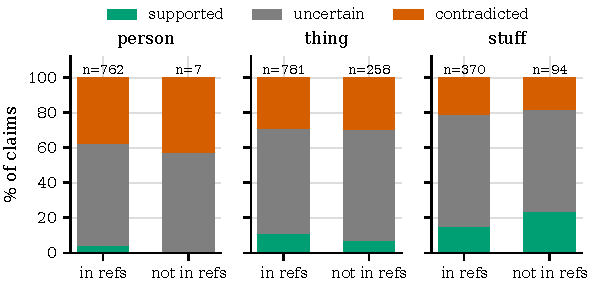
\includegraphics[width=\columnwidth]{figures/verdict_by_kind.pdf}
\caption{Verdicts of the attention-selected regions under the provisional thresholds, by claim kind and by whether a reference mentions the claimed class (raw attention).}
\label{fig:verdict}
\end{figure}

\subsection{Retell: Zero-Initialisation and First Training Runs}
\label{sec:exp-gate}
\textbf{Zero-initialisation.} Before the first update, every trained system reproduced the B0 draft exactly on the 200 validation images checked (\InitIdentical{} systems identical, beam search, same decoding settings). This holds by construction ($\tanh(0)=0$), but the check guards against implementation errors in the wrapped decoder. The pathway has \ParamsM\,M trainable parameters.

\textbf{First runs.} Table~\ref{tab:retell} reports one training run per system: three epochs on the half-B drafts with corruption rate $\rho=0.15$, evaluated on validation. These runs test that the full pipeline trains end to end and show how much the evidence moves the output. They are not tests of H1--H5, which need human labels and calibrated thresholds. These first runs used the earlier region rules and provisional thresholds. They establish an implementation baseline; they do not measure Retell performance with the frozen Look v2 records. Retell must be reassessed after Check calibration.

\begin{table*}[t]
\caption{Retell development runs on the validation split (decoder fine-tuned on A, pathway trained on B, 3 epochs,
$\rho=0.15$ unless stated). Each round has its own matched no-evidence control B0+. BLEU-4 and CIDEr use our
simplified tokeniser (compare only with scores using the same tokenisation). \emph{Changed}: captions that
differ from the draft. \emph{Alt.\ adopt.} / \emph{Con.\ kept}: of the draft claims whose record is
\emph{contradicted}, the share whose alternative label appears in the output / whose claimed label is still in
the output (the set of contradicted records depends on the thresholds, so these two columns are comparable only
within a round). \emph{Sens.}: captions that change when all evidence is masked. All columns are automatic;
none is a human-verified error rate.}
\label{tab:retell}
\centering\footnotesize
\begin{tabular}{@{}lccccccc@{}}
\toprule
System & BLEU-4 & CIDEr & RUOR & Changed (\%) & Alt.\ adopt.\ (\%) & Con.\ kept (\%) & Sens.\ (\%) \\
\midrule
B0 (draft) & 32.6 & 0.979 & 15.8 & -- & -- & -- & -- \\
B1 (word repl., provisional thr.) & 27.9 & 0.815 & 25.9 & 40.3 & -- & -- & -- \\
\midrule
\multicolumn{8}{@{}l}{\emph{Round 1: provisional thresholds, no patch dropout}} \\
B0+ (no evidence) & 34.0 & 0.983 & 15.7 & 63.6 & -- & -- & -- \\
LCR, raw attention & 34.2 & 0.987 & 15.8 & 65.0 & 15.1 & 90.3 & -- \\
LCR, sink-corr. attention & 34.3 & 0.991 & 15.7 & 64.1 & 41.0 & 87.1 & 10.9 \\
B3 (detector regions) & 34.1 & 0.981 & 15.8 & 64.6 & 26.5 & 88.8 & -- \\
B2 (image tags) & 34.3 & 0.983 & 15.7 & 64.7 & -- & -- & -- \\
\bottomrule
\end{tabular}
\end{table*}

\begin{table}[t]
\caption{Evidence interventions on validation: the same trained model with real records, all records masked
(null token only), or false records (alternative label of each contradicted record replaced by a class the
detector does not see in the image). \emph{Sens.}: captions that differ from the real-evidence output.
[R1]/[R2]: development round.}
\label{tab:interv}
\centering\footnotesize\setlength{\tabcolsep}{3pt}
\begin{tabular}{@{}p{2.3cm}lcccc@{}}
\toprule
System & Evidence & CIDEr & RUOR & Alt.\ adopt. & Sens.\ (\%) \\
\midrule
LCR, raw attention [R1] & real & 0.987 & 15.8 & 15.1 & -- \\
 & masked & 0.993 & 15.8 & 15.2 & -- \\
 & false & 0.987 & 15.8 & 0.0 & -- \\
\addlinespace
LCR, sink-corr. attention [R1] & real & 0.991 & 15.7 & 41.0 & -- \\
 & masked & 0.984 & 15.9 & 41.0 & 10.9 \\
 & false & 0.991 & 15.7 & 0.0 & 0.0 \\
\addlinespace
B3 (detector regions) [R1] & real & 0.981 & 15.8 & 26.5 & -- \\
 & masked & 0.990 & 15.7 & 27.6 & -- \\
 & false & 0.981 & 15.8 & 0.0 & -- \\
\bottomrule
\end{tabular}
\end{table}


\begin{figure}[t]
\centering
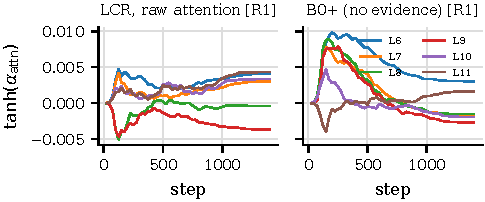
\includegraphics[width=\columnwidth]{figures/gate_curves.pdf}
\caption{Attention-gate values $\tanh(\alpha_{\text{attn}})$ of the six gated blocks during training, for LCR and for the no-evidence control B0+.}
\label{fig:gates}
\end{figure}

\subsection{Annotation Tool and Error Pilot}
The blinded annotation page (Section~\ref{sec:design-eval}) has been generated for the 100-image error pilot. It contains the B0 drafts of 100 randomly drawn validation images and asks for a label for every concrete noun, including nouns outside $V$. Labelling by two team members is the next step. Their labels will give the first human estimate of the draft error rate, Cohen's $\kappa$, and the data needed to set the verdict thresholds and fix the test sample size (Table~\ref{tab:power}).

\section{Summary and Next Steps}
\label{sec:conclusion}

\subsection{Work Done So Far}
Historical Look--Check--Retell variants and matched controls were implemented and run end to end. The current update unifies only Look and Check; new Retell training is explicitly deferred. Concretely, we have:
(i) built the claim vocabulary (\NumClasses{} classes, \NumSurface{} surface forms) and the extraction rules;
(ii) cached BLIP and OWLv2 features for the training and validation images, including the per-proposal scale and shift that make detector scores reproducible for any later query;
(iii) fine-tuned the drafting decoder on half A (validation CIDEr \ZsCIDEr{} $\to$ \FtCIDEr{});
(iv) generated drafts, attention maps and verification records for half B and the validation split;
(v) trained the Retell pathway and the B0+, B2 and B3 controls once each, and verified that the zero-initialised pathway reproduces the draft exactly before training;
(vi) built the blinded annotation tool and the scoring code for HICR, fix/break/NRR, $\kappa$ and bootstrap intervals.

\subsection{What the Results So Far Show}
\begin{itemize}
\item Reference agreement is a poor proxy for correctness, especially for \emph{thing} and \emph{stuff} claims. This supports the decision to make human judgement the primary measure.
\item BLIP's raw cross-attention is not a usable localisation signal because of attention sinks. A gradient-free sink correction raises human-box pointing accuracy from \LookRawPoint\% to \LookSinkPoint\%. The bounded E1 refinement raises region accuracy from v2's \LookVTwoRegion\% to frozen v3's \LookClosedRegion\%. E2 adds no source under the predefined acceptance rule. Feature-level interventions show greater sensitivity to Look-selected than matched random token masks; this is not a pixel-level causal claim.
\item With provisional thresholds the detector contradicts far too many correct claims. Calibrating the verdict thresholds on human labels is required before B1 and before the final Retell training.
\item The power analysis shows that H1 is only testable with a paired, claim-traced design, and only if the draft error rate is not much below 8\%.
\end{itemize}

\subsection{Deviations from the Proposal}
We fine-tune only the BLIP decoder (encoder frozen), cache two additional OWLv2 quantities, label claims by kind, take corruption labels from the captioner's own runner-up words, and use sink-corrected instead of raw attention. Each change is justified in Section~\ref{sec:design}. The timeline is roughly on track: the work planned for weeks 1--7 is done except the human labelling and threshold calibration, which have moved into the next phase.

\subsection{Next Steps}
Table~\ref{tab:plan} lists the remaining work. The critical path runs through the pilot labels. Whether S4's operating point is right, the test sample size $N$ and the final Retell training all depend on them.

\begin{table}[t]
\caption{Remaining plan (weeks refer to the proposal's 12-week schedule).}
\label{tab:plan}
\centering\footnotesize
\begin{tabular}{@{}p{1.1cm}p{6.6cm}@{}}
\toprule
Week & Task \\
\midrule
8 & Label the stratified B pilot (a random group plus S4/S2 decision groups; two annotators, an adjudicator, $\kappa$): S4's real precision, substitute accuracy and removal harm, misidentified vs.\ invented errors and referent boxes; fix $N$ from the random group's error rate; audit Flickr30k Entities phrase mappings for H6. \\
9 & Run the Look L1 measurements and decide on abstention; re-run B1 on S4's replacements; give Retell Check's action and substitute; retrain LCR, B0+, B2, B3 and the $\rho\in\{0,0.15,0.3\}$ ablation with sink-corrected attention; select epochs on a held-out part of training half B. \\
10 & Reversed split (decoder on B, Retell on A); COCO Karpathy-test inference and CHAIR for all systems (H1b). \\
11 & Blinded human evaluation on the test sample (HICR, CCI, fix/break/NRR); H4 screening and interventions; H6 localisation with gradient relevance as an alternative. \\
12 & Statistics (paired bootstrap, sign tests), limitations, final report. \\
\bottomrule
\end{tabular}
\end{table}

\textbf{Main risks.} (1) If the pilot shows a draft error rate well below 8\%, H1 will be underpowered even with the paired design. In that case COCO CHAIR (H1b) becomes the main factuality evidence, as the proposal foresaw. (2) If Retell keeps ignoring the evidence after calibration, H4 will document it. Raising $\rho$ and giving B3's detector-selected regions as an alternative input are the planned responses. (3) Human annotation is the main workload, and the deduplicated annotation tool is ready for it.


\section*{Team Contributions}
\textbf{\.{I}.~G\"{o}zl\"{u}kaya}: BLIP fine-tuning, draft generation, synthetic corruption, Retell and B0+ training, coordination.
\textbf{\.{I}.~Billurcu}: evidence encoder, null token, gated layers, B2.
\textbf{M.~C.~Ayd\i{}n}: claim extraction, attention localisation and coordinate mapping, OWLv2 caching and verification, B1/B3.
\textbf{Z.~B.~Deniz}: automatic metrics, CHAIR, evidence interventions, power analysis.
\textbf{D.~Kemal}: human-evaluation protocol and annotation tool, error pilot.
All members contributed to the literature review and to writing.

\bibliographystyle{IEEEtran}
\bibliography{refs}

\end{document}
